% =================================================

\begin{frame}
\frametitle{Data Sources}
\framesubtitle{Overview of Traffic Light Control (Ampelbeeinflussung)}
\begin{figure}
\centering
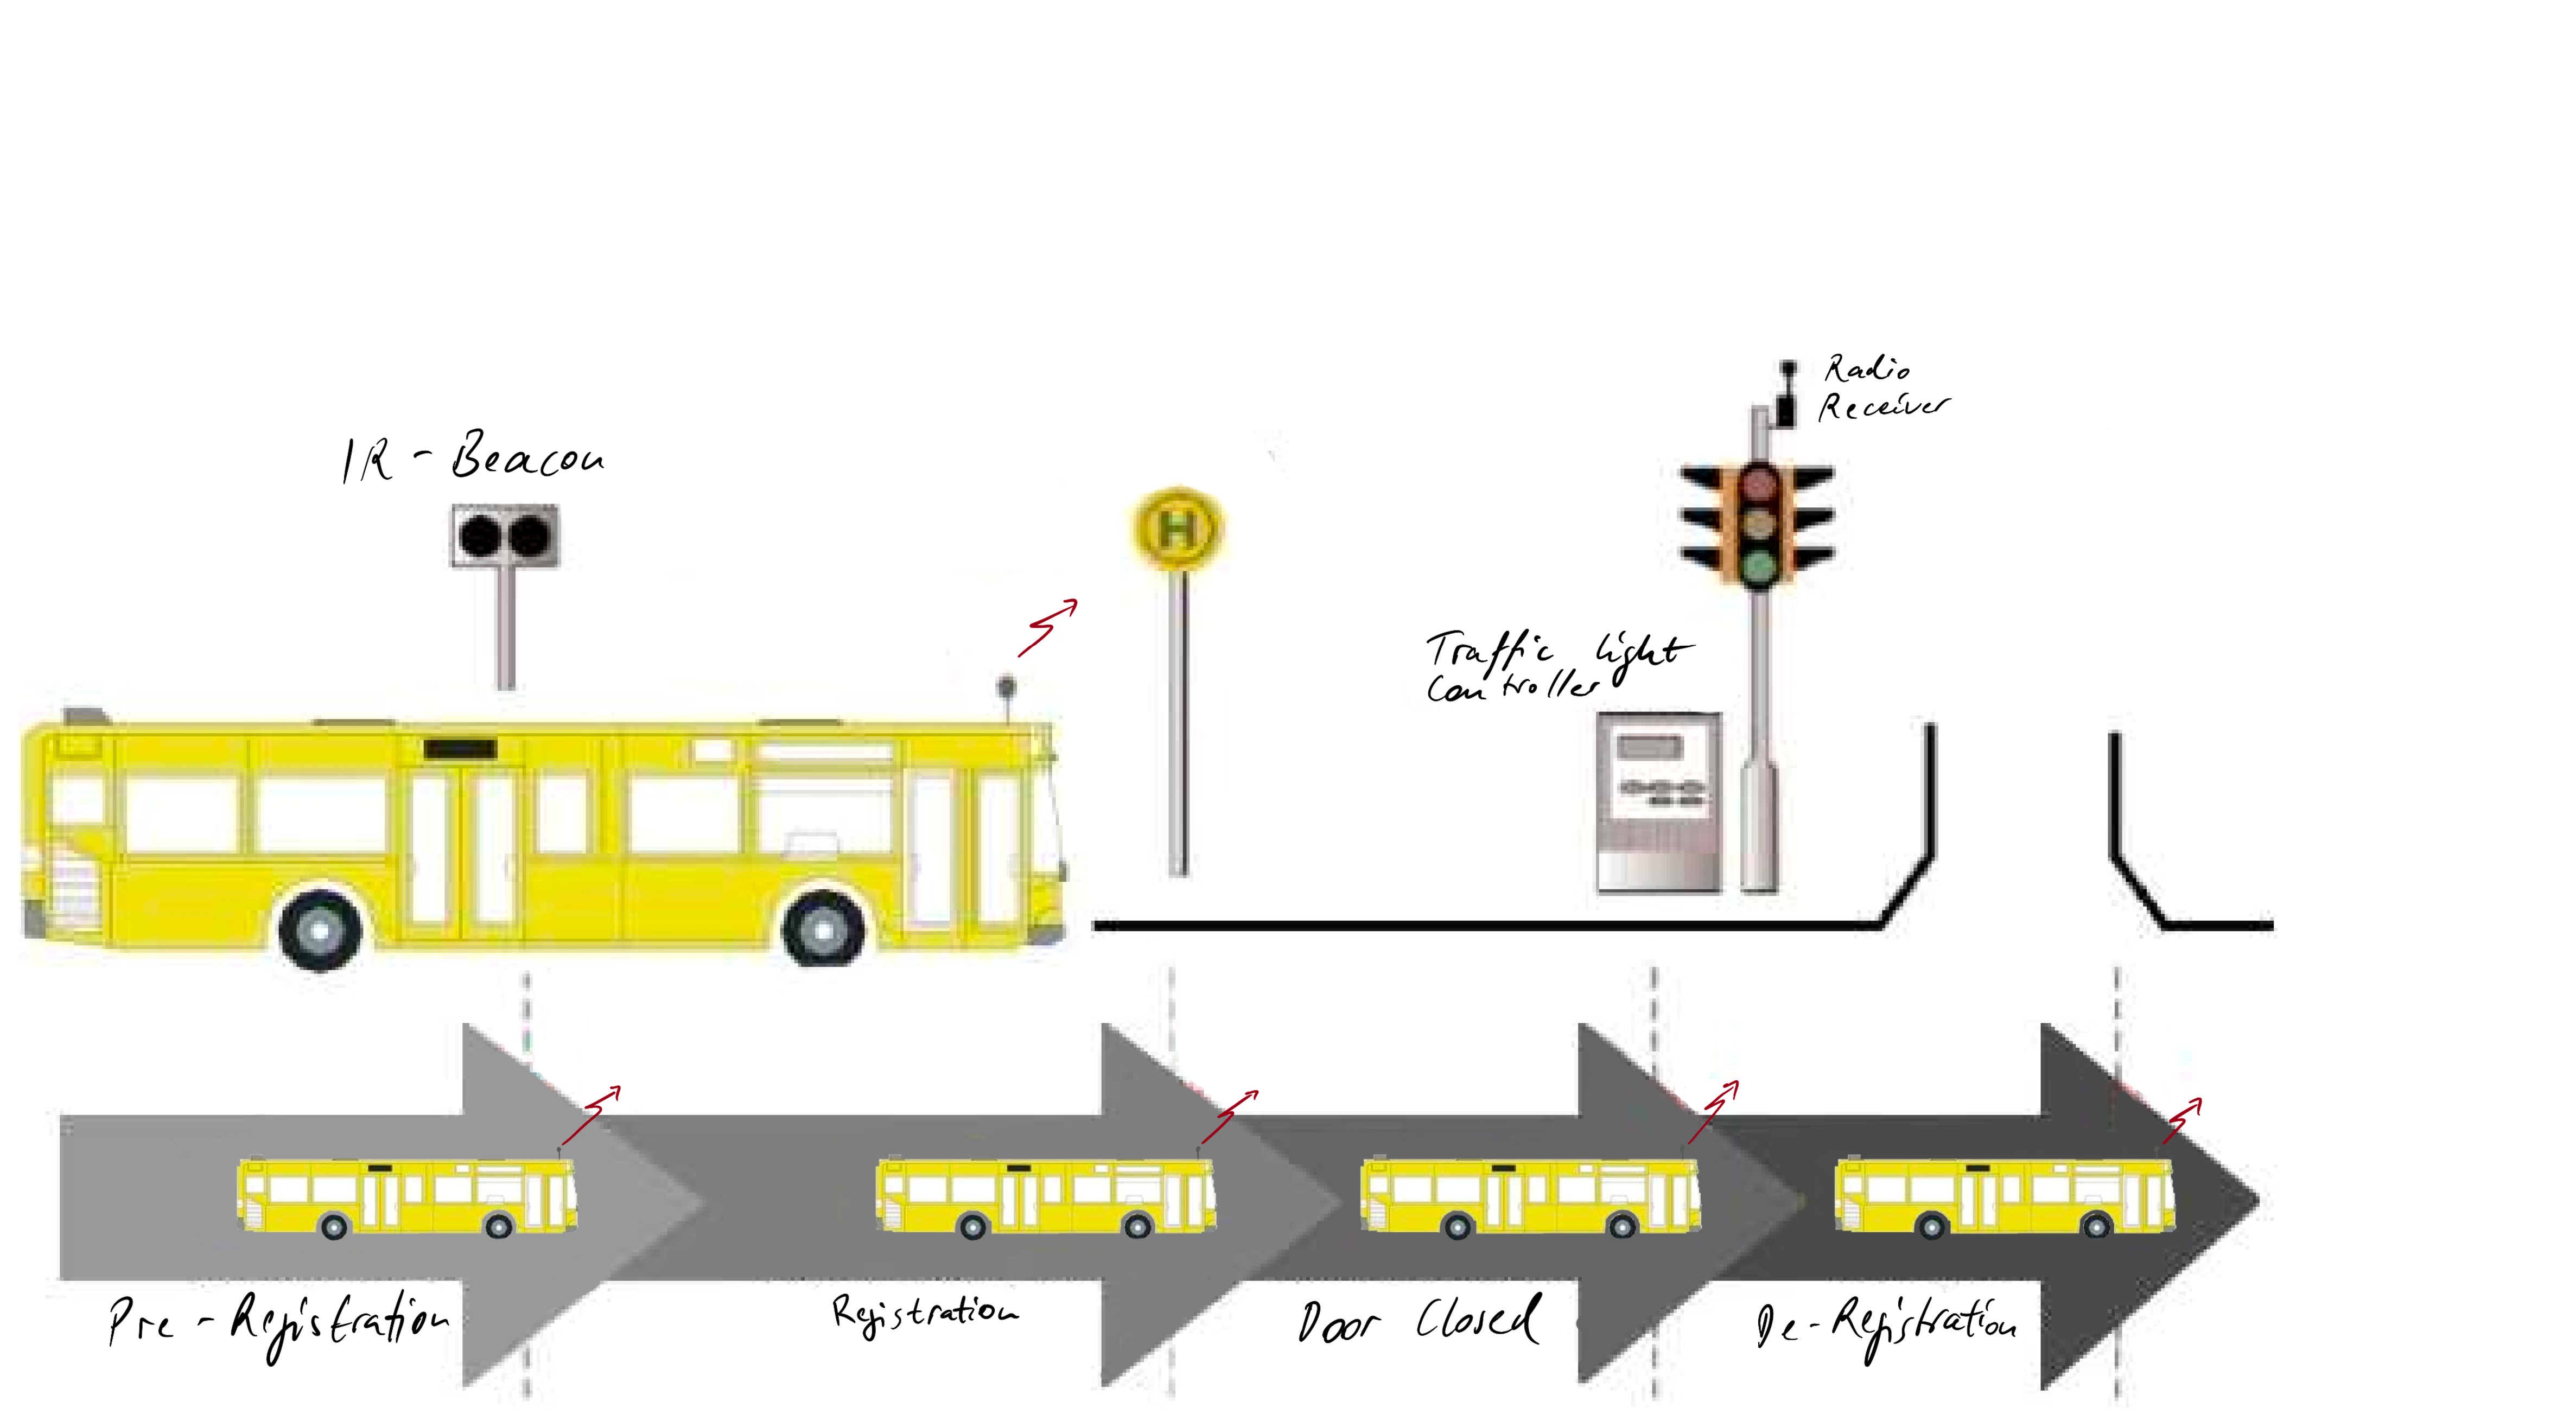
\includegraphics[height=0.65\textheight]{figs/lsa-beeinflussungs-stecke.pdf}
\caption{Traffic light controlled by radio link of busses and trams. Modified graphic from \Colorhref{https://urbic-system.com/wp-content/uploads/2020/10/Qualitaetssicherung-an-Lichtsignalanlagen-aus-Sicht-des-OEPNV-im-urbanen-Umfeld-Kopie.pdf}{urbic}}
\end{figure}
\end{frame}

% =================================================

\begin{frame}
\frametitle{Data Sources}
\framesubtitle{Overview of Traffic Light Control (Ampelbeeinflussung)}
\begin{figure}
\centering
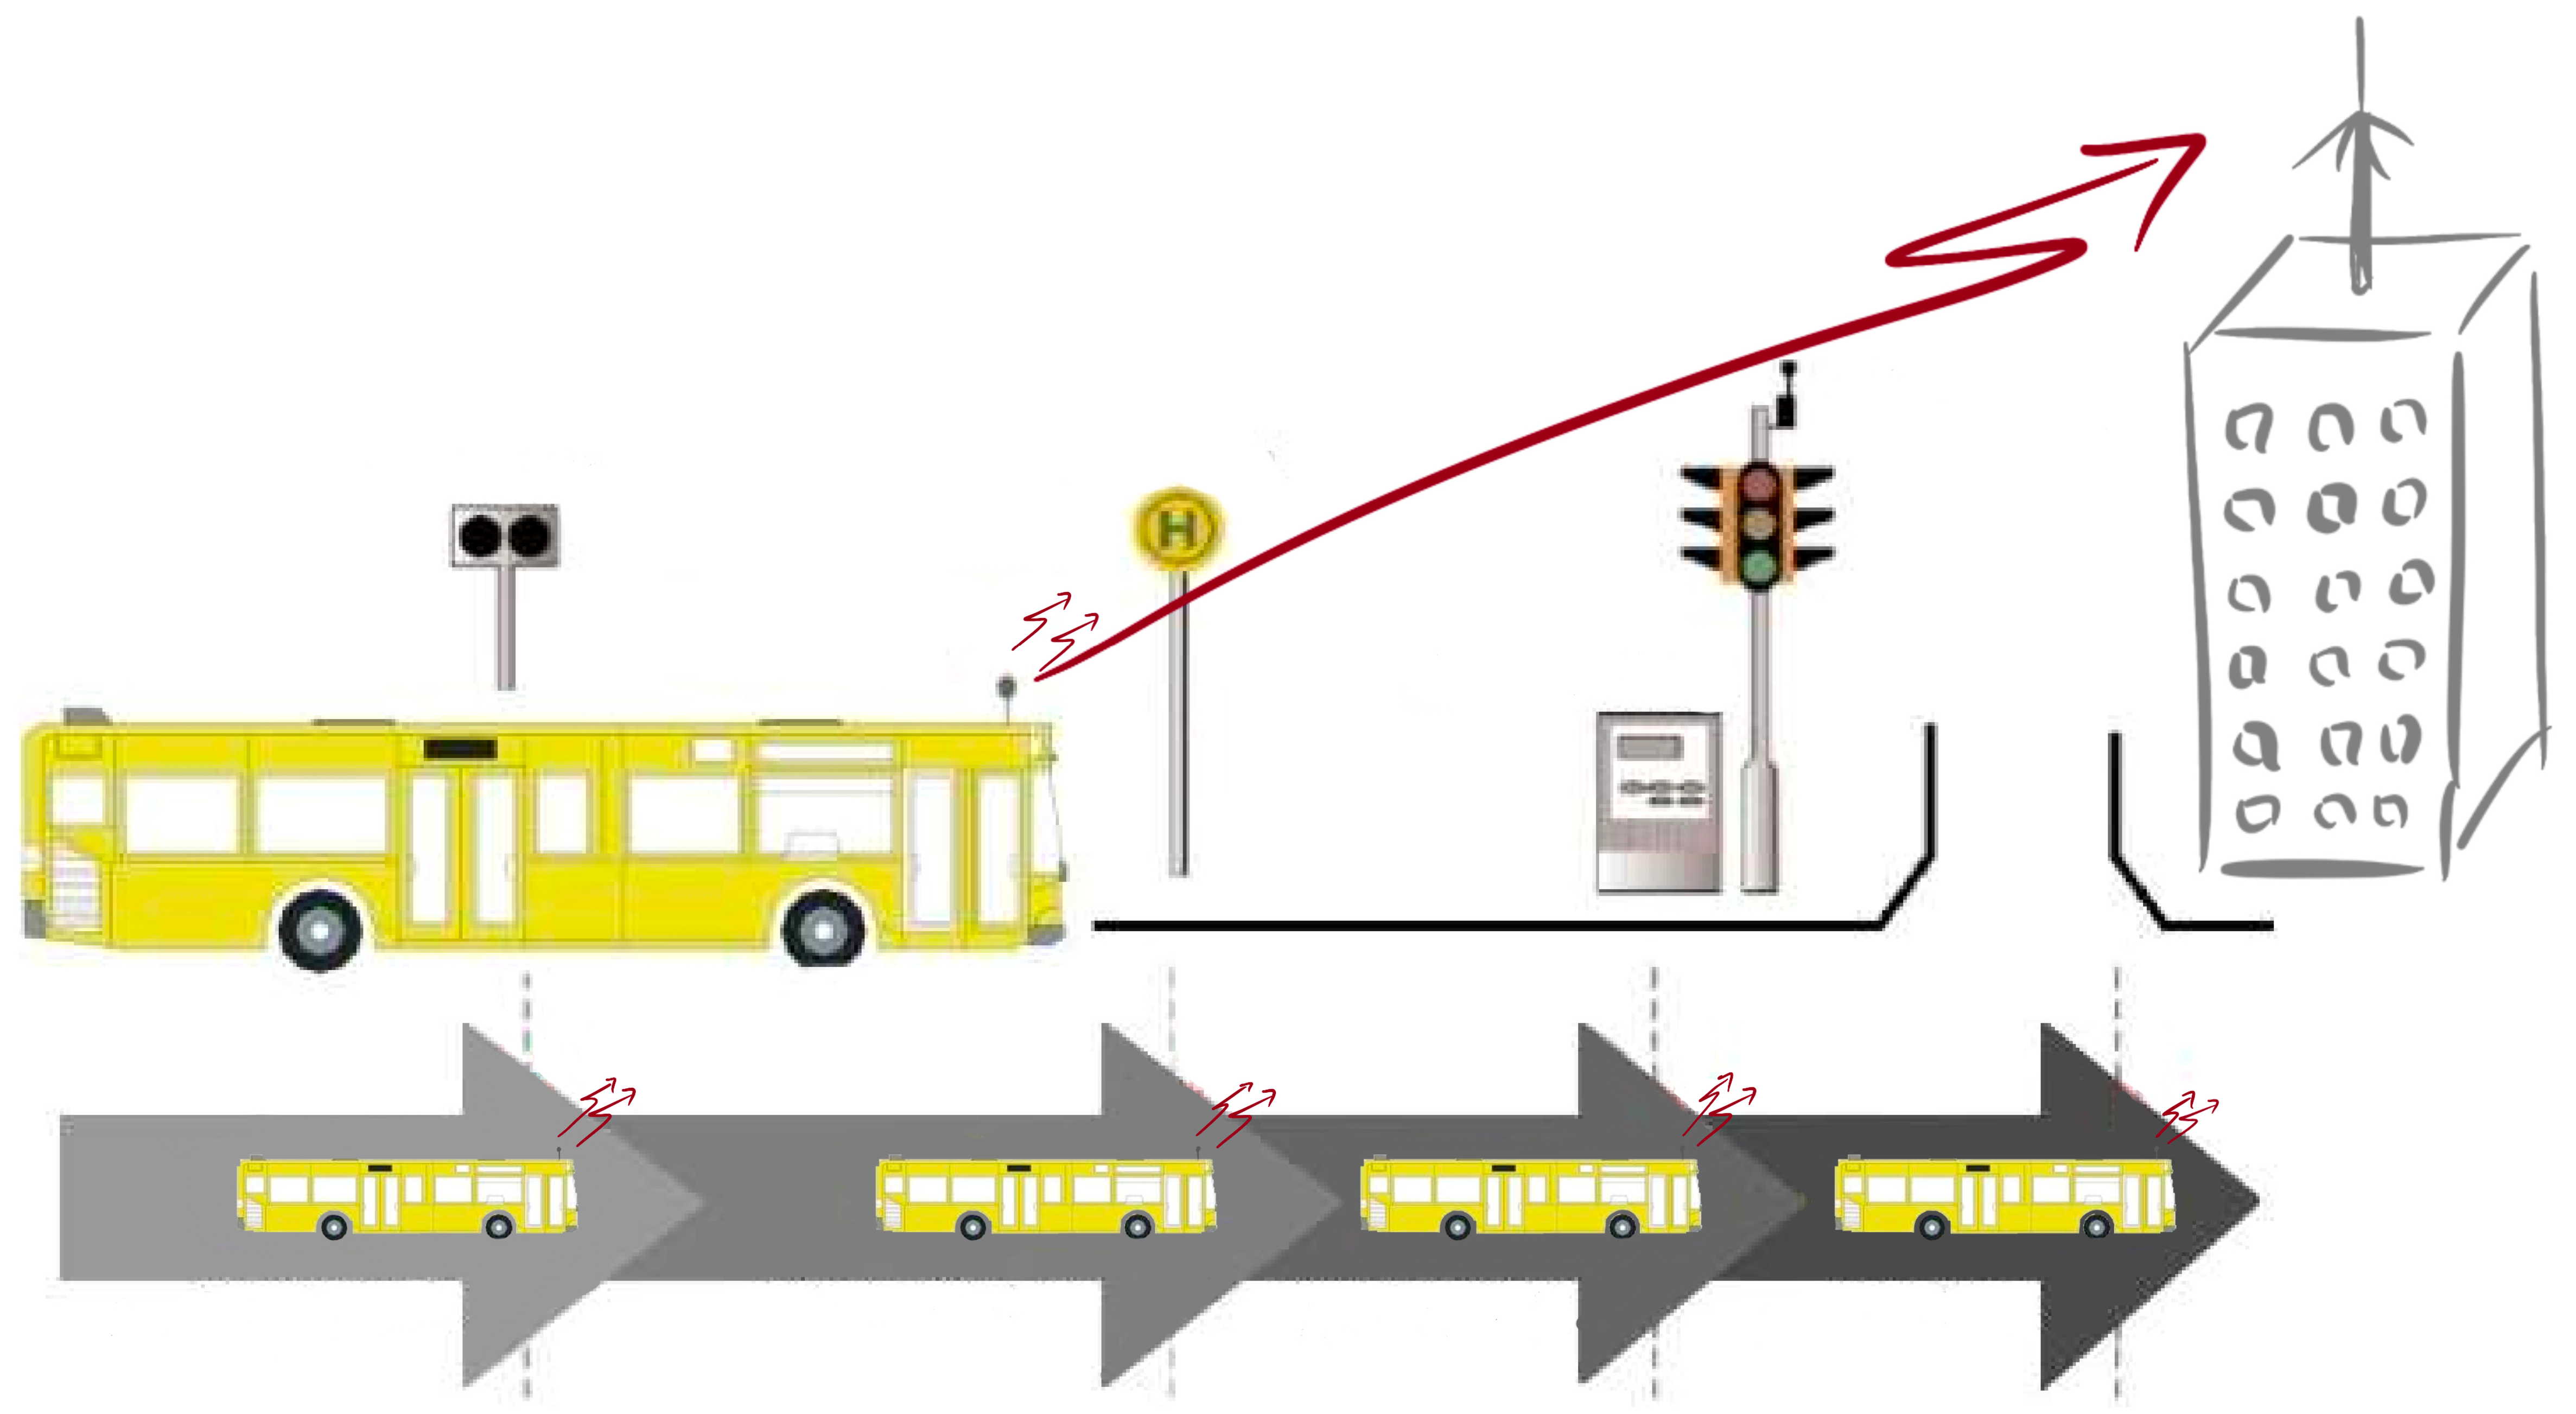
\includegraphics[height=0.65\textheight]{figs/lsa-beeinflussungs-stecke-mit-antenne.pdf}
\caption{Radio signals can be received by our antennas}
\end{figure}
\end{frame}

% =================================================

\begin{frame}
\frametitle{Data Sources}
\framesubtitle{Receiver Overview}
\begin{figure}
\centering
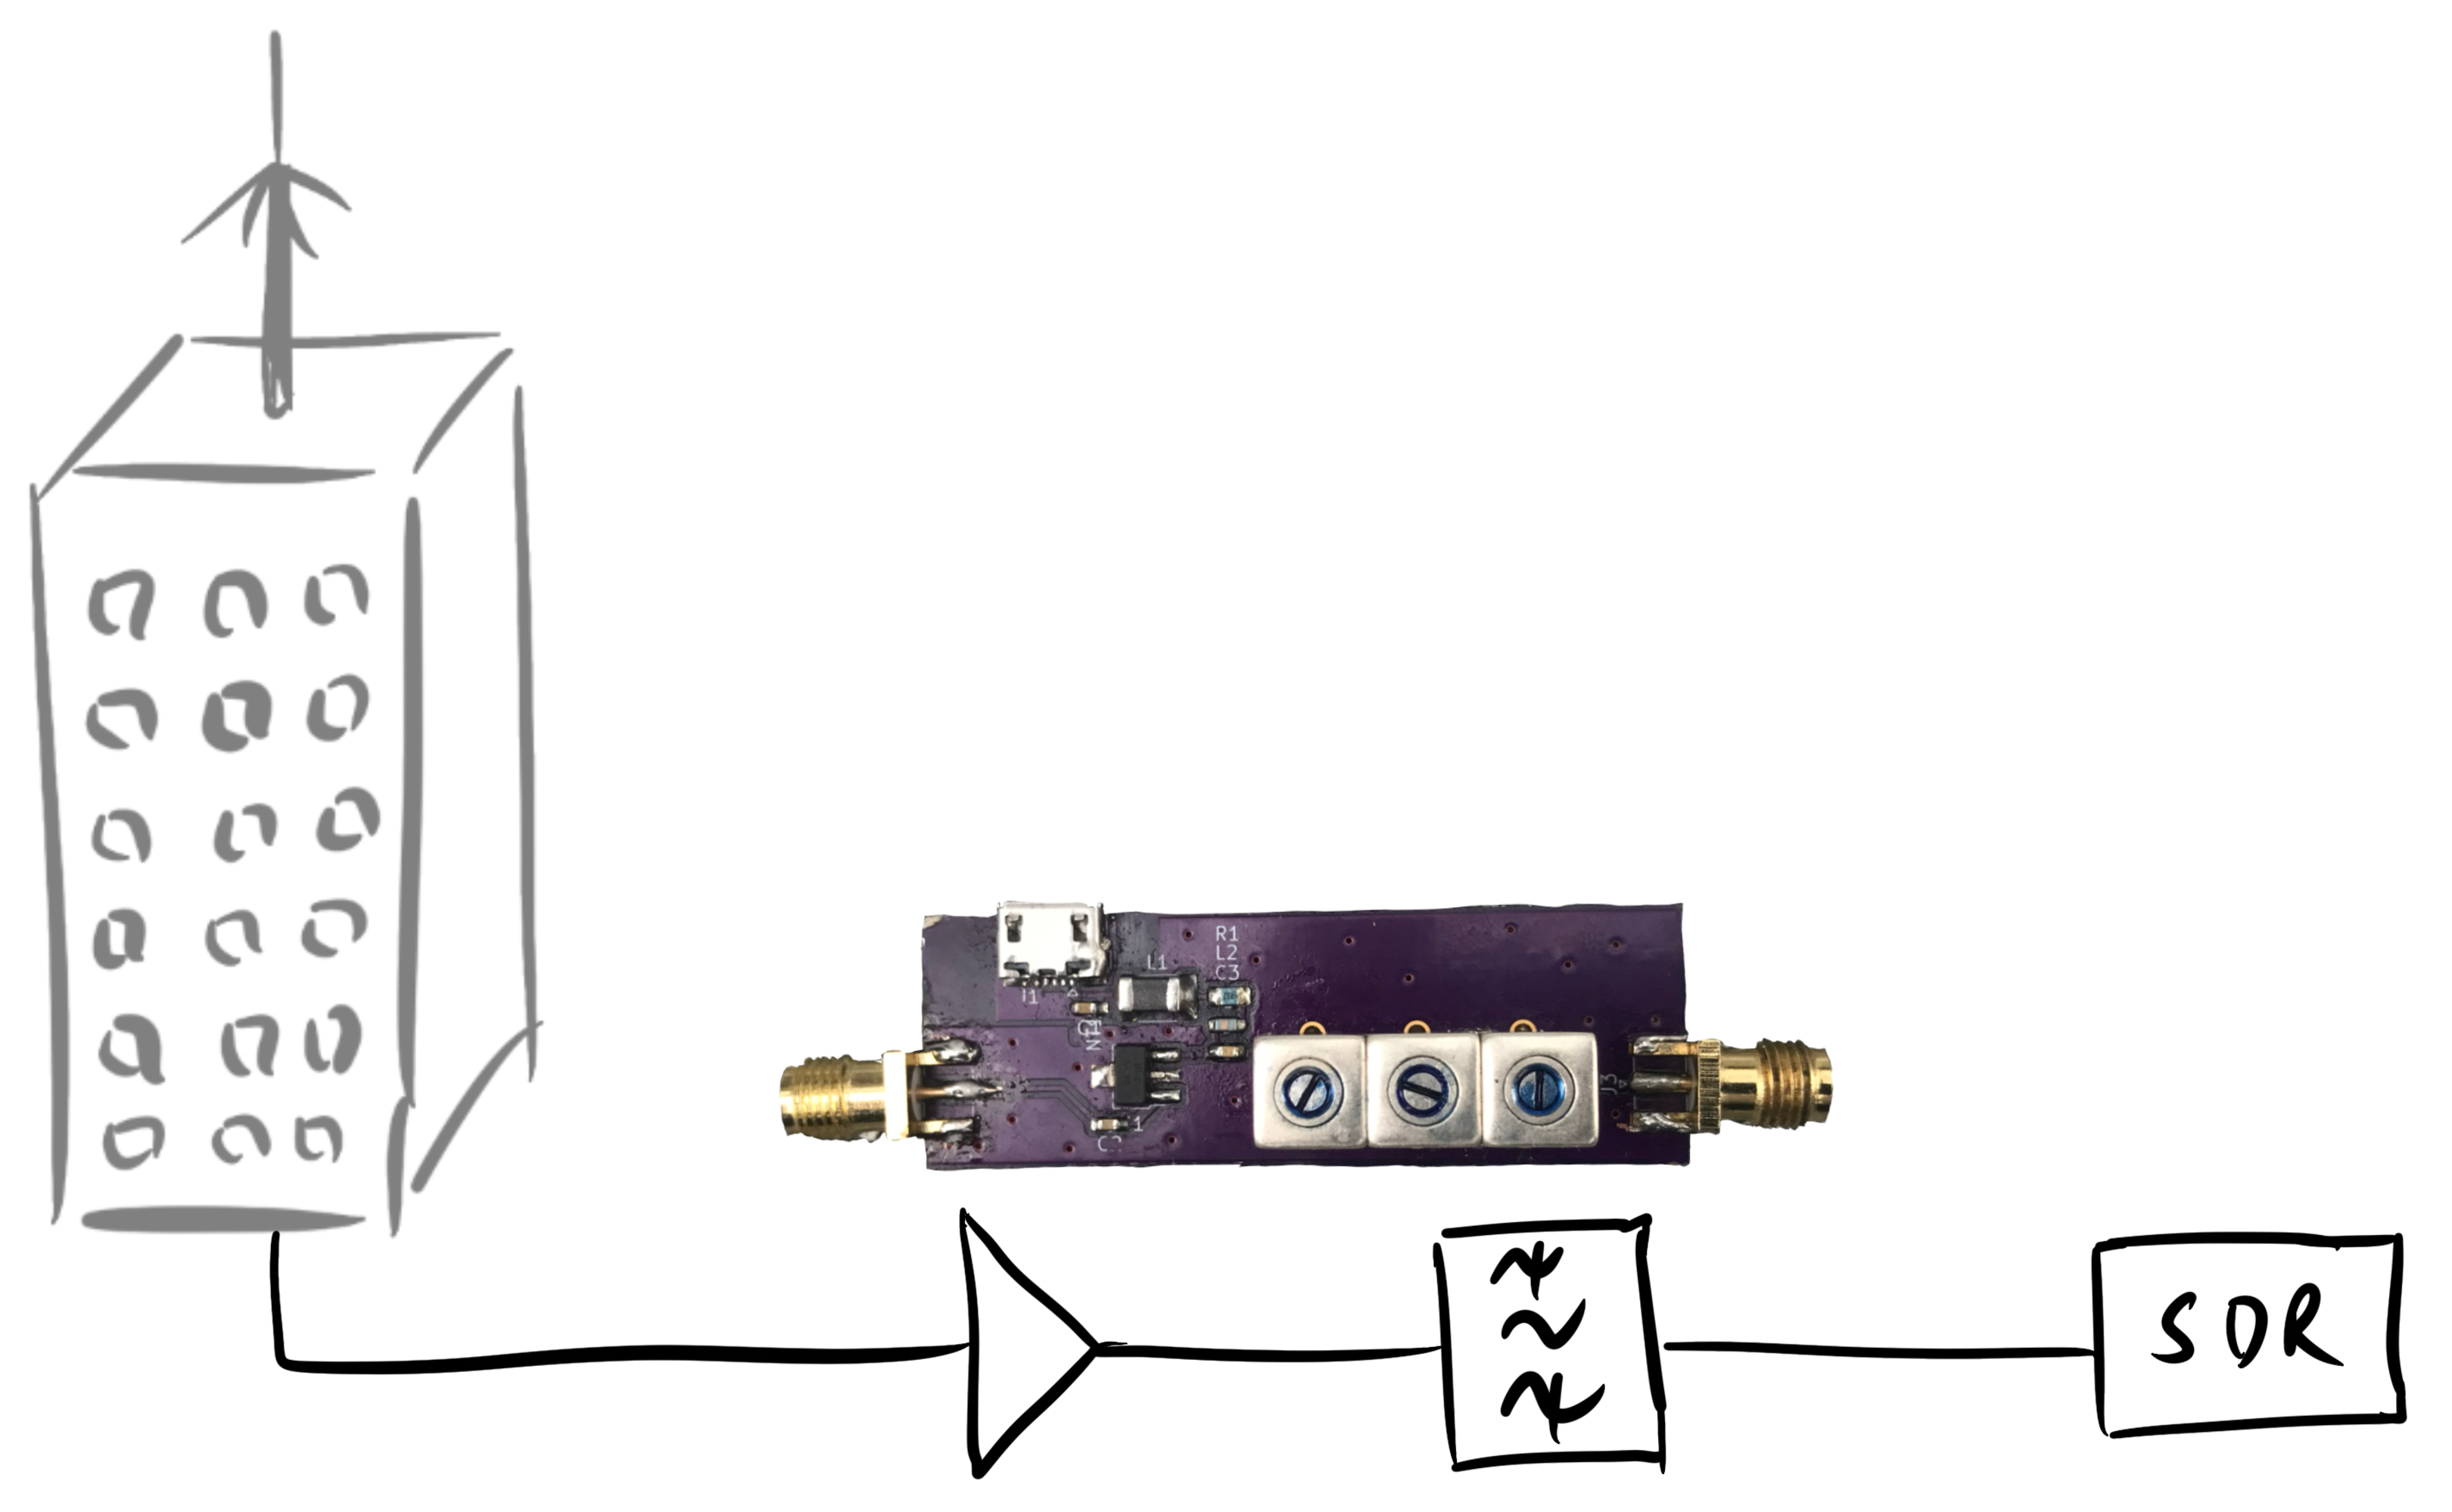
\includegraphics[height=0.65\textheight]{figs/antenna-filter.pdf}
\caption{Schematic overview of the receiver hardware}
\end{figure}
\end{frame}

% =================================================

\begin{frame}
\frametitle{Protocol}
\framesubtitle{VDV 420}
\todo[inline]{This slide is a big todo}
	\begin{itemize}
%		\item which protocol?
%		\item which frequency?
		\item some background on Ampelbeeinflussung and VDV 420 / 426
		\item R09 telegrams of trams and busses standardized in \Colorhref{https://knowhow.vdv.de/documents/420/}{VDV 420}
	\end{itemize}
\end{frame}

% =================================================

\begin{frame}
\frametitle{Protocol}
\framesubtitle{VDV 420 Data}
\begin{itemize}
	\item What data do we receive?
	\begin{itemize}
		\item Tram identification: line number (3 decimal digits), run number (2 decimal digits), destination number (3 digits)
		\item Location: Reporting point (16 bit) which might contain 2 bit registration\_type (Pre-registration, Registraion, De-registration, Doors closed), traffic light id and direction
		\item Other data: Delay ($\pm 7$), train length (until now always zero) etc.
	\end{itemize}
	\item Representation of data might be different than in the original standard
	% https://www.tirol.gv.at/fileadmin/themen/verkehr/verkehrsplanung/Verkehrsmanagement/Downloads/101022_PRL_VLSA-Tirol_V1.1_inkl_Anh01-Anh10.pdf
	\todo[inline]{represantion of dresden/tirol}
	\todo[inline]{screenshot from vdv 426}
\end{itemize}
\end{frame}

% =================================================

\begin{frame}
\frametitle{Protocol}
\framesubtitle{VDV 420 Physical Layer}
\begin{columns}
\column{0.6\linewidth}
\centering
\begin{figure}
\centering
\begin{subfigure}[b]{0.46\textwidth}
	\centering
	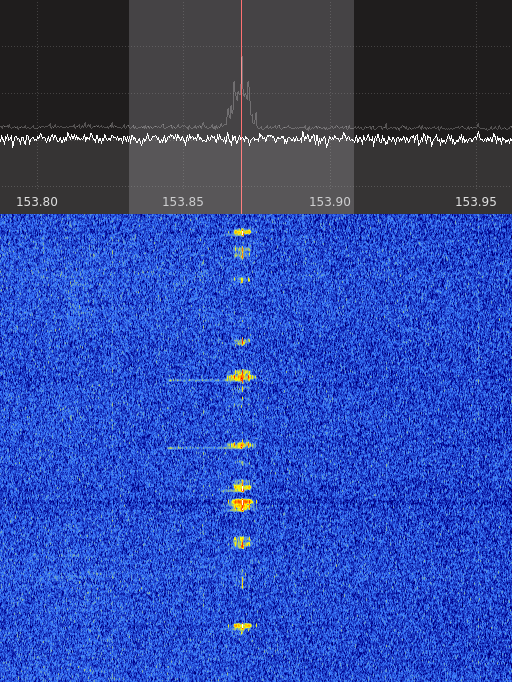
\includegraphics[height=0.65\textheight,width=\textwidth]{figs/spectrum_chemnitz_cropped.png}
\end{subfigure}
\hfill
\begin{subfigure}[b]{0.46\textwidth}
	\centering
	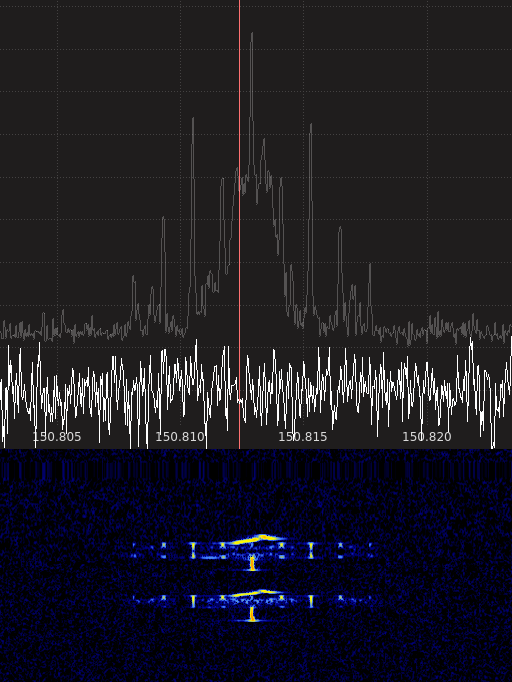
\includegraphics[height=0.65\textheight,width=\textwidth]{figs/spectrum_dresden_cropped.png}
\end{subfigure}
\caption{Screenshots of the bursty transmittion pattern}
\end{figure}
\column{0.4\linewidth}
\begin{itemize}
	\item Bursty transmittion
	\item Minimum Shift Keying with \SI{2400}{Baud}
\end{itemize}
\end{columns}
\end{frame}

% =================================================

\begin{frame}
\frametitle{Protocol}
\framesubtitle{Frequency Identification}
\begin{columns}
\column{.276\linewidth}
\centering
\begin{figure}
	\centering
	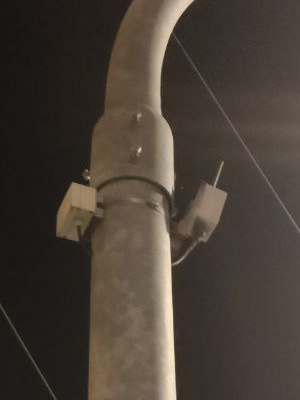
\includegraphics[width=\textwidth]{figs/lsa-antenna.png}
	\caption{Telegram receiver on the right}
\end{figure}
\column{.724\linewidth}
\begin{itemize}
		\item What are the frequency ranges to look for the signal?
		\item Technical documentation of different receivers, i.e. \Colorhref{https://www.piciorgros.com/fileadmin/documents/RBL380.pdf}{RBL-380} or \Colorhref{https://www.img-nordhausen.de/wp-content/uploads/2021/05/DA\_WZLSA\_2-3\_G\_d\_03\_15.pdf}{WZ LSA 2-3/G}, provide these details
		\item Frequency 70cm Band \SI{450}{\MHz} -- \SI{470}{\MHz}		
		\item Frequency 2m Band \SI{146}{\MHz} -- \SI{174}{\MHz}
		\item Frequency 4m Band \SI{68}{\MHz} -- \SI{87.5}{\MHz}
		\item We have a \Colorhref{https://docs.dvb.solutions/chapter\_3\_data\_providers.html}{table of known frequencies}
		\item OSINT: Search for ``R09 frequency <city>''
\end{itemize}
\end{columns}
\end{frame}

% =================================================

\begin{frame}
\frametitle{Protocol}
\framesubtitle{Physical Layer Used in Different Cities}
\begin{figure}
% https://opus4.hbz-nrw.de/opus45-bast/frontdoor/deliver/index/docId/2595/file/V353+BF+Gesamtversion.pdf
% page 25
\begin{columns}
\column{.5\linewidth}
\centering
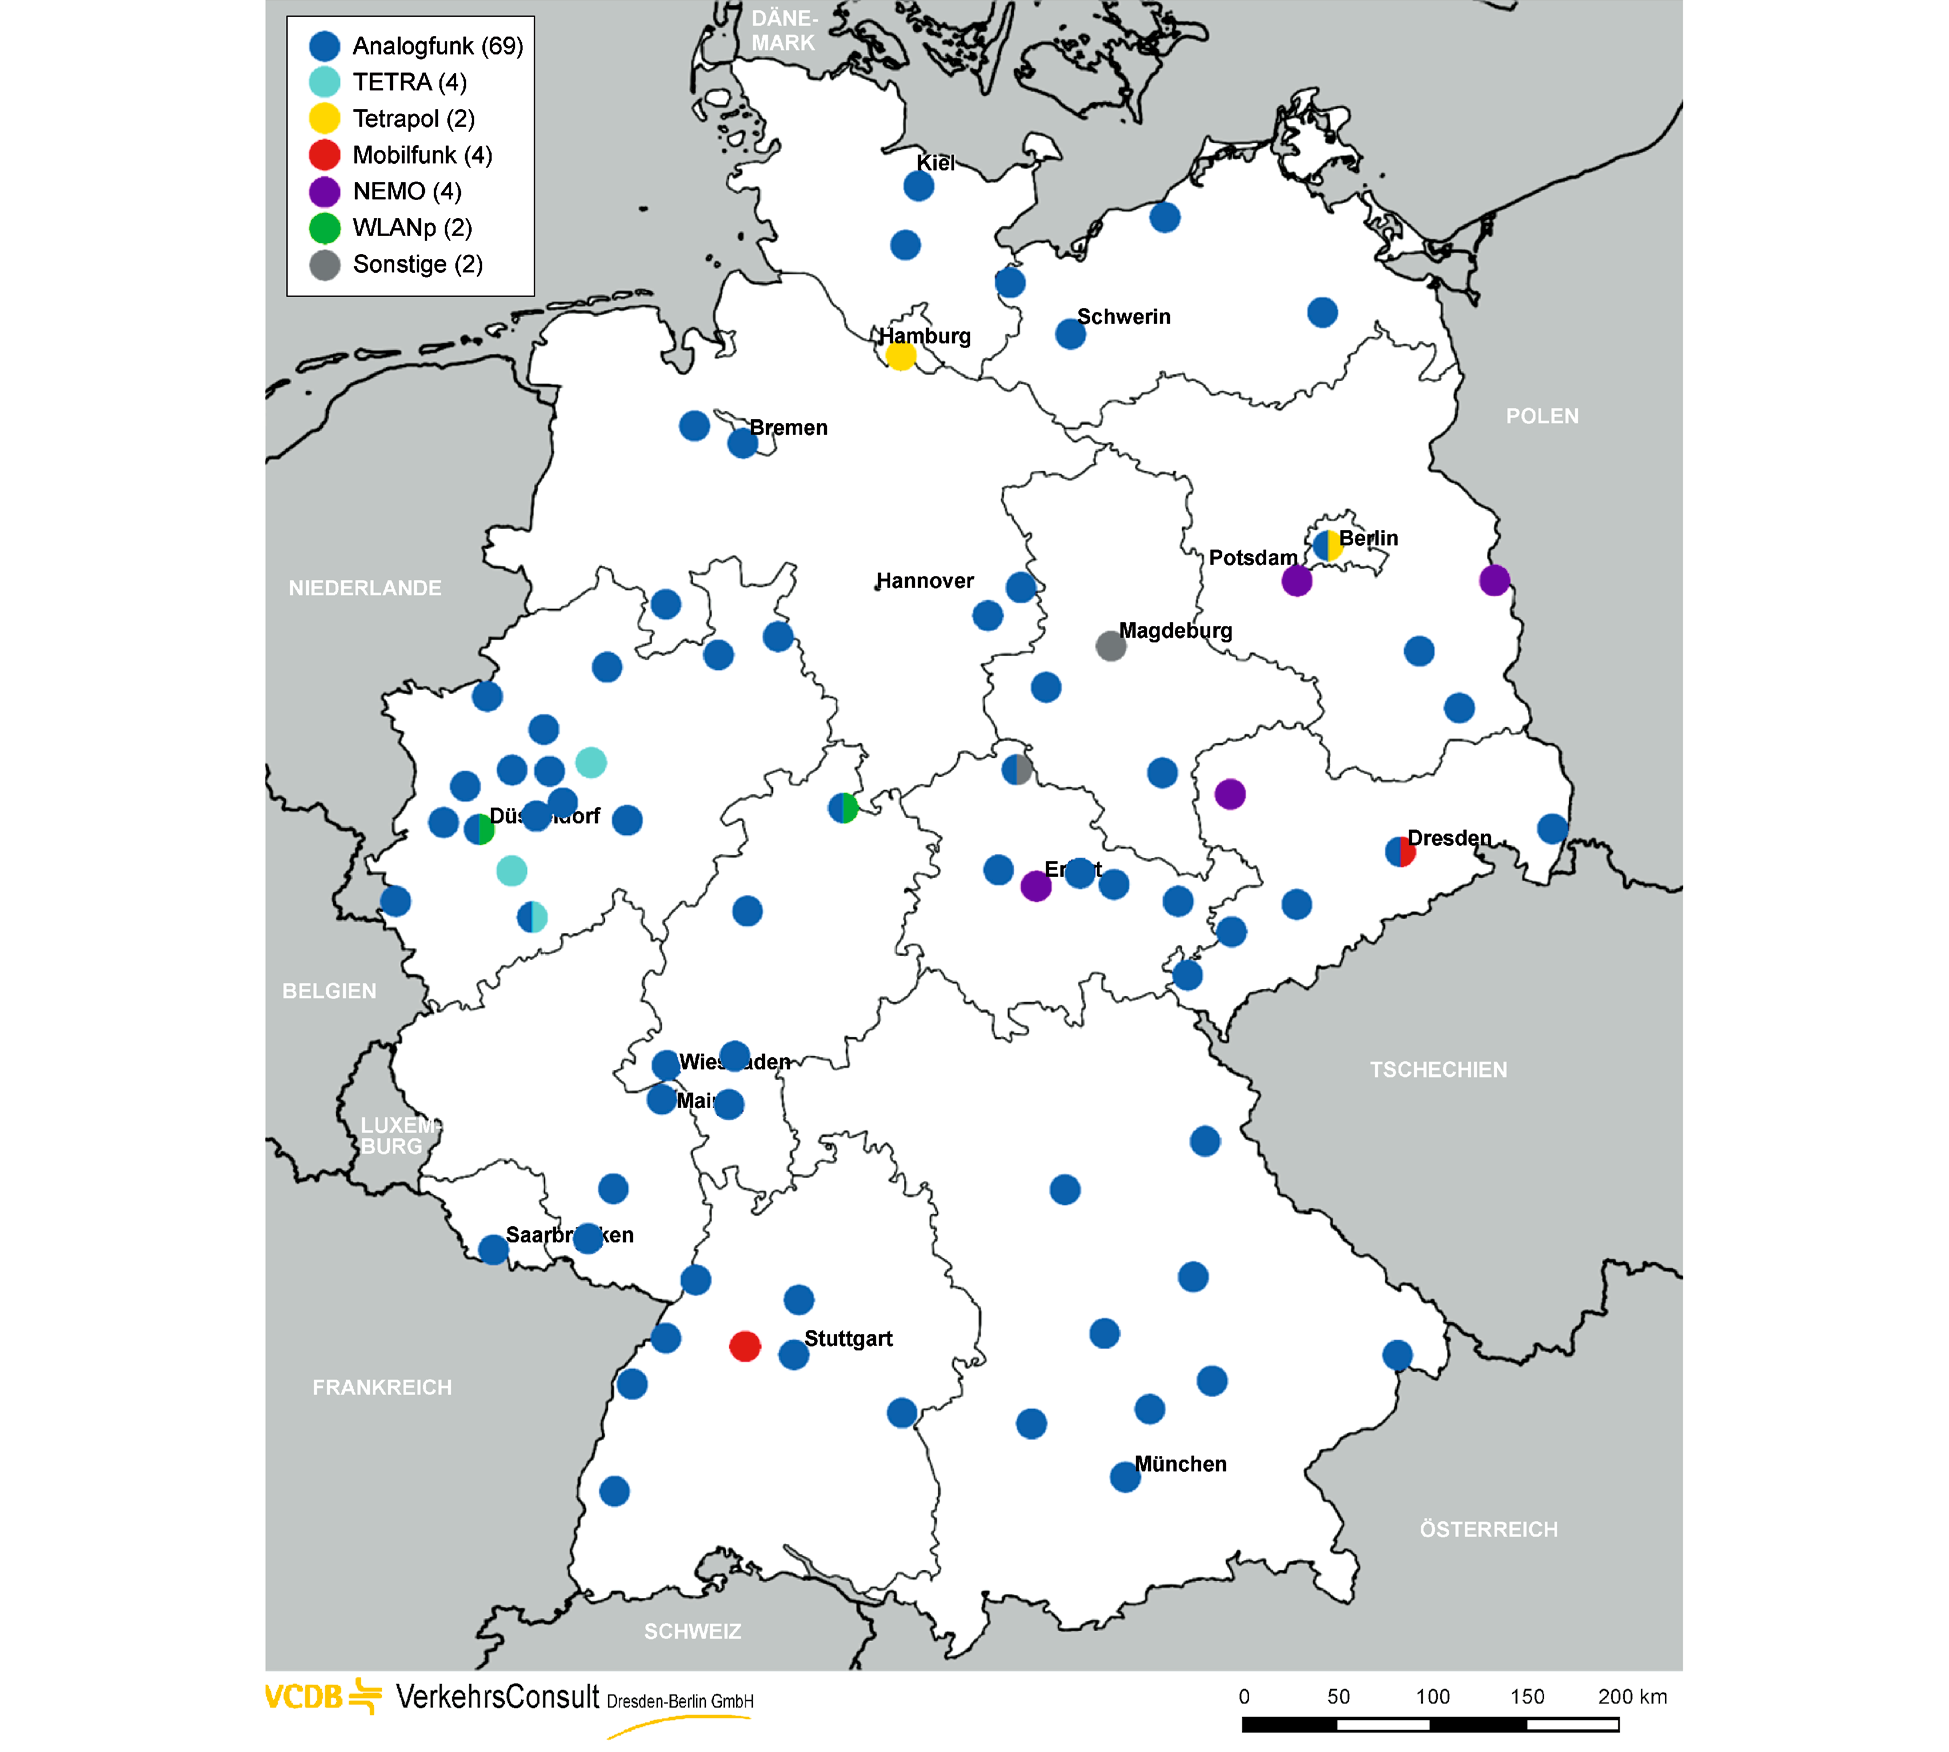
\includegraphics[height=0.8\textheight]{figs/vcdb-map-ampelbeeinflussung.png}
\column{.5\linewidth}
\caption{Map with selected locations which have traffic lights, controlled by public transport. Blue points use the standard we implemented.}
\vspace{0.5cm}
\begin{itemize}
	\item Implementations using a different physical layer exsist too, i.e. Berlin with Tetrapol
	\item \Colorhref{https://knowhow.vdv.de/documents/426/}{VDV 426} has more information on this topic
	\item Actual included data doesn't seem to be different
\end{itemize}
\todo[inline]{add link for the map}
\end{columns}
\end{figure}
\end{frame}

% =================================================
